\section{Results}

\subsection{Operator performance and accuracy}

Table~\ref{tab:primary-results} is the primary comparison. Panel A places the
same finite NV/MX route on our GB200 and B300 systems and adds HAO's published
GB300 NV/FP8 result where the shape matches. Panel B reproduces HAO's complete
D128 grid locally on GB200 and reports both TK policies against one BF16
reference. Unbounded shiftless NV/NV timings are excluded even when a
particular input happens to be finite.

\begin{table}[htbp]
\centering
\caption{Primary performance and accuracy comparison. Panel A contains local
TK measurements; bold marks independently confirmed B300 results above
3 PFLOP/s. Panel B uses identical Q/K/V and BF16 outputs for both TK policies.
Published HAO columns are cross-run context. ``ms / TF'' means milliseconds
and TFLOP/s; TK error is cosine / relative-$L_2$ against BF16.}
\label{tab:primary-results}
\begingroup
\scriptsize
\setlength{\tabcolsep}{3pt}
\renewcommand{\arraystretch}{0.92}

\textbf{A. Retained TK NV/MX across generations}\par\smallskip
\begin{adjustbox}{max width=\textwidth}
\begin{tabular}{lccccc}
\toprule
Shape & TK GB200 ms / TF & TK B300 ms / TF & HAO GB300 NV/FP8 TF / cos.
& B300 $\Delta$t & TK B300 cosine / rel.-$L_2$ \\
\midrule
D128/H24/S4096 & 0.092160 / 2237 & 0.087008 / 2369 & 2046 / 0.9898 & -5.59\% & 0.9438 / 0.3363 \\
D128/H64/S4096 & 0.202752 / 2711 & 0.189536 / 2901 & -- & -6.52\% & 0.9440 / 0.3355 \\
D128/H64/S6144 & 0.452848 / 2731 & 0.418107 / 2958 & -- & -7.67\% & 0.9432 / 0.3381 \\
D128/H64/S8192 & 0.758336 / 2900 & \textbf{0.705684 / 3116} & -- & -6.94\% & 0.944063--0.944113 / 0.334931--0.335152 \\
D128/H64/S9472 & -- & \textbf{0.930724 / 3159} & -- & -- & 0.943960--0.944056 / 0.335198--0.335473 \\
D128/H24/S32768 & 4.400448 / 2998 & 4.480736 / 2945 & 2677 / 0.9899 & +1.82\% & 0.9429 / 0.3389 \\
D64/H24/S4096 & 0.097888 / 1053 & 0.093248 / 1105 & -- & -4.74\% & 0.9556 / 0.2967 \\
D64/H64/S4096 & 0.221184 / 1243 & 0.207840 / 1323 & -- & -6.03\% & 0.9558 / 0.2960 \\
D64/H24/S32768 & 4.863296 / 1357 & 4.601808 / 1434 & 1203 / 0.9892 & -5.38\% & 0.9561 / 0.2950 \\
D64/H64/S32768 & 12.865536 / 1367 & 12.223360 / 1439 & -- & -4.99\% & 0.9572 / 0.2915 \\
\bottomrule
%
\end{tabular}
\end{adjustbox}

\vspace{3pt}
\textbf{B. Complete published HAO D128 grid}\par\smallskip
\begin{adjustbox}{max width=\textwidth}
\begin{tabular}{lcccccccc}
\toprule
Shape & TK NV/MX fast & Error & TK NV/MX accurate & Error
& HAO B200 & HAO GB300 & HAO cosine & HAO GB300 \\
 & ms / TF & cos. / rel.-$L_2$ & ms / TF & cos. / rel.-$L_2$
& NV/FP8 TF & NV/FP8 TF & NV/FP8 & BF16 TF \\
\midrule
B1/S256/H16/D128 & 0.010560 / 51 & 0.9445 / 0.3367 & 0.012288 / 44 & 0.9527 / 0.3242 & 39 & 11 & 0.9904 & 17 \\
B1/S1024/H16/D128 & 0.016704 / 514 & 0.9441 / 0.3357 & 0.018432 / 466 & 0.9519 / 0.3268 & 416 & 203 & 0.9901 & 289 \\
B1/S4096/H12/D128 & 0.064480 / 1599 & 0.9434 / 0.3376 & 0.077888 / 1323 & 0.9515 / 0.3287 & 1118 & 1458 & 0.9899 & 1017 \\
B1/S4096/H24/D128 & 0.092160 / 2237 & 0.9440 / 0.3358 & 0.110528 / 1865 & 0.9519 / 0.3266 & 1548 & 2046 & 0.9898 & 1322 \\
B4/S4096/H16/D128 & 0.200992 / 2735 & 0.9436 / 0.3370 & 0.248384 / 2213 & 0.9514 / 0.3279 & 1875 & 2502 & 0.9899 & 1508 \\
B4/S4096/H32/D128 & 0.391168 / 2811 & 0.9436 / 0.3367 & 0.489280 / 2247 & 0.9514 / 0.3277 & 1920 & 2540 & 0.9898 & 1475 \\
B1/S32768/H12/D128 & 2.279968 / 2893 & 0.9443 / 0.3348 & 2.867520 / 2301 & 0.9518 / 0.3262 & 1913 & 2582 & 0.9896 & 1584 \\
B1/S32768/H16/D128 & 2.964512 / 2967 & 0.9429 / 0.3387 & 3.726912 / 2360 & 0.9508 / 0.3295 & 2016 & 2666 & 0.9897 & 1585 \\
B1/S32768/H24/D128 & 4.400448 / 2998 & 0.9438 / 0.3364 & 5.461024 / 2416 & 0.9516 / 0.3275 & 2018 & 2677 & 0.9899 & 1533 \\
\bottomrule
%
\end{tabular}
\end{adjustbox}
\endgroup
\end{table}

Across the nine GB200 D128 rows, \code{fast} is
\HaoGridFastGeoSpeedup$\times$ faster than HAO BF16 geometrically and peaks
at \HaoGridFastPeakTflops\ TFLOP/s. \code{Accurate} reaches
\HaoGridAccurateGeoSpeedup$\times$ and \HaoGridAccuratePeakTflops\ TFLOP/s.
At S32768/H24, fast takes 4.400448 ms (2998 TFLOP/s), compared with HAO's
published 2018 TFLOP/s on B200 and 2677 TFLOP/s on GB300 for NV/FP8.

HAO NV/FP8 remains more accurate: its mean cosine is
\HaoPublishedMeanCosine, versus \HaoGridFastMeanCosine\ for fast and
\HaoGridAccurateMeanCosine\ for accurate. The corresponding TK mean
relative-$L_2$ values are \HaoGridFastMeanRelLTwo\ and
\HaoGridAccurateMeanRelLTwo. HAO does not publish relative-$L_2$ for these
rows. Appendix~\ref{app:accuracy-matched-control} measures the cost of matching
its cosine with our exact NV/FP8 route; the local HAO NV/NV and full format
matrix remain in Appendices~\ref{app:nvnv} and \ref{app:format-matrix}.

B300 improves D128 latency by 5.6--7.7\% on the S4096--S8192 rows in Panel A.
The standard S8192/H64 case reaches \BThreeThreeKStandardTflops\ TFLOP/s,
and wave-aligned S\BThreeThreeKPeakSeq/H64 reaches
\BThreeThreeKPeakTflops\ TFLOP/s. The exception is S32768/H24: B300 reaches
2945 TFLOP/s versus 2998 on GB200. D64 shows a 4.7--6.0\% B300 latency gain
on the displayed rows. At HAO's published shapes, our B300 NV/MX reaches 2369
versus 2046 TFLOP/s at S4096/H24/D128, 2945 versus 2677 at
S32768/H24/D128, and 1434 versus 1203 at S32768/H24/D64. These are different
implementations and harnesses, so they establish scale rather than causal
timing differences.

\subsection{Speed--accuracy behavior across shapes}

Figure~\ref{fig:headline-pareto} shows the independent B1/S4096/H24/D128
suite, including optimized local FP8-PV controls. Its six-order reference
harness produces slightly different timings from Table~\ref{tab:primary-results},
but all points share one BF16 value.

\begin{figure}[htbp]
\centering
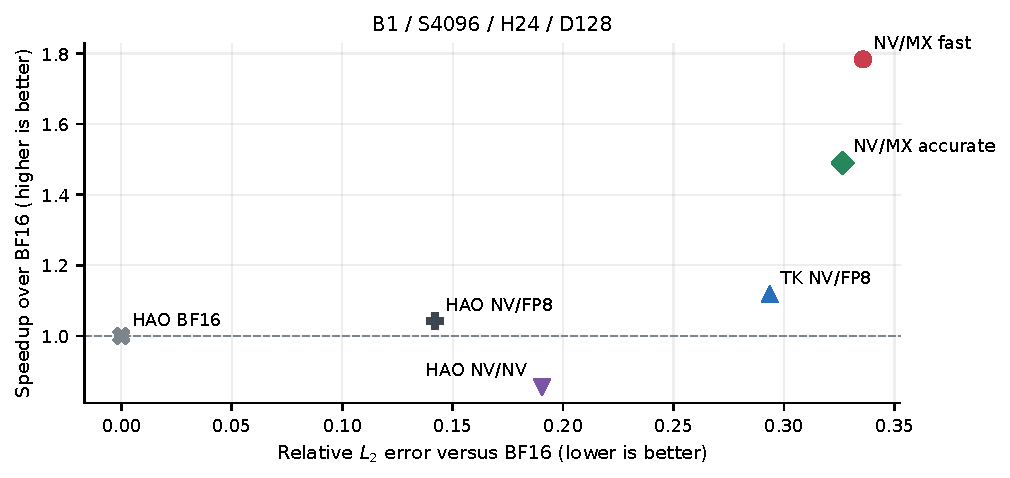
\includegraphics[width=.83\textwidth]
  {../fp4_fa4_unified_20260801/figures/headline_pareto.pdf}
\caption{Speed--error plane for the headline shape. Up and left are better.
The fastest full-FP4 points accept more operator error than HAO NV/NV or FP8
PV.}
\label{fig:headline-pareto}
\end{figure}

FP8 PV avoids the E2M1 payload and block-scale page required by full FP4 and
is more accurate. The local TK NV/FP8 control reaches only 1.118$\times$ BF16
in this suite, whereas NV/MX fast reaches 1.783$\times$; HAO's stronger
published NV/FP8 result is therefore included in the primary table rather
than inferred from this local control.

Figure~\ref{fig:cross-shape} adds H64 cases. At S4096/H64, fast takes
0.202752 ms versus 0.370688 ms for BF16 (1.828$\times$). At S8192/H64 it
takes 0.758336 ms versus 1.611488 ms (2.125$\times$). The two-query CTA is
important here: the earlier one-query topology created twice as many jobs and
could require an additional GPU wave at high head count.

\begin{figure}[htbp]
\centering
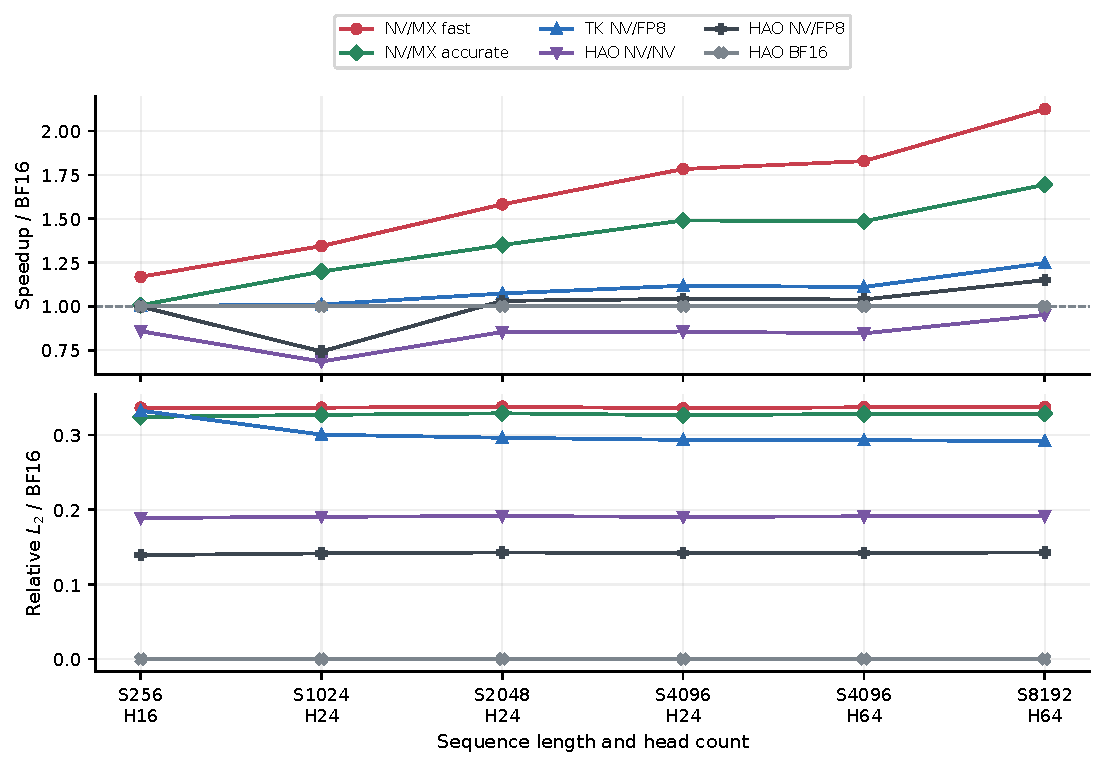
\includegraphics[width=.96\textwidth]
  {../fp4_fa4_unified_20260801/figures/cross_shape_speed_accuracy.pdf}
\caption{BF16 speedup and relative-$L_2$ from matched records across startup,
transition, and saturated shapes.}
\label{fig:cross-shape}
\end{figure}

\subsection{ViT and BERT replays}

Table~\ref{tab:downstream-tradeoff} joins physical attention speed, mean layer
error, and final task behavior. ViT uses 1,000 examples at S256 and 200 at
S1024/S4096. BERT MLM uses 800 S256 blocks and 200 S512 blocks; SST-2 uses all
872 validation examples.

\begin{table}[htbp]
\centering
\caption{Downstream replay trade-off. Task score is provider / BF16 accuracy.
Final and layer cells are cosine / relative-$L_2$ against BF16. Speedup belongs
to the physical attention shape, not the complete model. HAO NV/NV is the
identical-input control because no NV/FP8 task replay is published.}
\label{tab:downstream-tradeoff}
\scriptsize
\begin{adjustbox}{max width=\textwidth}
\begin{tabular}{llrrrrrr}
\toprule
Task & Provider & Speedup & Task score / BF16 (\%) & Agree. (\%)
& Final cos. / rel.-$L_2$ & Layer cos. / rel.-$L_2$ & $\Delta$MLM loss \\
\midrule
ViT S256 & TK NV/MX \code{fast} & 1.169$\times$ & 98.80 / 98.90 & 99.30 & 0.9987 / 0.0514 & 0.9885 / 0.1506 & -- \\
ViT S256 & TK NV/MX \code{accurate} & 1.007$\times$ & 98.70 / 98.90 & 99.60 & 0.9990 / 0.0452 & 0.9902 / 0.1401 & -- \\
ViT S256 & HAO NV/NV & 0.858$\times$ & 98.70 / 98.90 & 99.80 & 0.9997 / 0.0238 & 0.9961 / 0.0872 & -- \\
ViT S1024 & TK NV/MX \code{fast} & 1.344$\times$ & 95.00 / 96.50 & 97.50 & 0.9971 / 0.0768 & 0.9938 / 0.1093 & -- \\
ViT S1024 & TK NV/MX \code{accurate} & 1.198$\times$ & 97.00 / 96.50 & 99.50 & 0.9984 / 0.0564 & 0.9949 / 0.1001 & -- \\
ViT S1024 & HAO NV/NV & 0.685$\times$ & 97.00 / 96.50 & 99.50 & 0.9995 / 0.0324 & 0.9978 / 0.0652 & -- \\
ViT S4096 & TK NV/MX \code{fast} & 1.783$\times$ & 88.50 / 88.50 & 95.50 & 0.9887 / 0.1509 & 0.9961 / 0.0886 & -- \\
ViT S4096 & TK NV/MX \code{accurate} & 1.490$\times$ & 89.00 / 88.50 & 98.50 & 0.9989 / 0.0479 & 0.9971 / 0.0776 & -- \\
ViT S4096 & HAO NV/NV & 0.856$\times$ & 88.00 / 88.50 & 98.00 & 0.9992 / 0.0396 & 0.9986 / 0.0517 & -- \\
BERT SST-2 S256 & TK NV/MX \code{fast} & 1.169$\times$ & 92.32 / 92.43 & 98.74 & 0.9963 / 0.0870 & 0.9360 / 0.3547 & -- \\
BERT SST-2 S256 & TK NV/MX \code{accurate} & 1.007$\times$ & 92.09 / 92.43 & 98.74 & 0.9967 / 0.0815 & 0.9507 / 0.3045 & -- \\
BERT SST-2 S256 & HAO NV/NV & 0.858$\times$ & 92.20 / 92.43 & 99.77 & 0.9991 / 0.0431 & 0.9789 / 0.1890 & -- \\
BERT MLM S256 & TK NV/MX \code{fast} & 1.169$\times$ & 61.26 / 61.74 & 90.61 & 0.9968 / 0.0796 & 0.9740 / 0.2302 & +0.035 \\
BERT MLM S256 & TK NV/MX \code{accurate} & 1.007$\times$ & 61.36 / 61.74 & 91.11 & 0.9971 / 0.0758 & 0.9768 / 0.2170 & +0.028 \\
BERT MLM S256 & HAO NV/NV & 0.858$\times$ & 61.60 / 61.74 & 93.06 & 0.9983 / 0.0577 & 0.9864 / 0.1626 & +0.016 \\
BERT MLM S512 & TK NV/MX \code{fast} & 1.344$\times$ & 61.10 / 61.79 & 90.17 & 0.9969 / 0.0782 & 0.9763 / 0.2176 & +0.037 \\
BERT MLM S512 & TK NV/MX \code{accurate} & 1.198$\times$ & 61.36 / 61.79 & 90.83 & 0.9971 / 0.0761 & 0.9779 / 0.2104 & +0.040 \\
BERT MLM S512 & HAO NV/NV & 0.685$\times$ & 61.28 / 61.79 & 92.30 & 0.9982 / 0.0604 & 0.9861 / 0.1636 & +0.028 \\
\bottomrule
%
\end{tabular}
\end{adjustbox}
\end{table}

Both NV/MX policies remain finite. On ViT S4096, fast matches BF16 top-1
accuracy (88.5\%) with 95.5\% prediction agreement; accurate reaches 89.0\%
and 98.5\%, while native HAO NV/NV reaches 88.0\% and 98.0\%. Fast improves
from roughly 0.944 cosine in the Gaussian operator test to 0.9961 mean layer
cosine on this model input. Residual paths, normalization, later mixing, and
decision margins can attenuate operator error, so standalone relative-$L_2$
is informative but is not itself a task loss.

Across \DownstreamClassificationSamples\ classification examples, fast
changes \DownstreamFastPredictionChanges\ predictions, with
\DownstreamFastLowMarginChanges\ in the lowest quartile of BF16 top-two logit
margins. All changes from accurate and HAO NV/NV also lie in that quartile.
This supports a margin mechanism, but the suite is too small to establish
universal inference or training safety.

\subsection{Wan video diffusion}

Wan is a larger, native-shape test: all video self-attention calls run at
S7680/D128, while text cross-attention and the rest of the model stay BF16.
Table~\ref{tab:wan-downstream} compares every route with paired HAO CuTe-DSL
BF16 outputs and warmed kernel timing.

\begin{table}[htbp]
\centering
\caption{Wan2.1 quality and warmed GB200 kernel speed at S7680/D128. Speedup
is relative to HAO CuTe-DSL BF16. Quality is cosine / relative-$L_2$ of the
final latent against the paired BF16 run.}
\label{tab:wan-downstream}
\scriptsize
\begin{adjustbox}{max width=\textwidth}
\begin{tabular}{llrrccc}
\toprule
Model & Method & Time (ms) & Speedup & 1 step & 4 steps & 20 steps \\
\midrule
Wan2.1-1.3B & HAO CuTe BF16 & 0.2888 & 1.00$\times$ & 1.0000 / 0.0000 & 1.0000 / 0.0000 & 1.0000 / 0.0000 \\
Wan2.1-1.3B & TK NV/MX fast & 0.1653 & 1.75$\times$ & 0.9870 / 0.1803 & 0.9671 / 0.2611 & 0.9136 / 0.4163 \\
Wan2.1-1.3B & TK NV/MX accurate & 0.1961 & 1.47$\times$ & 0.9862 / 0.1721 & 0.9654 / 0.2637 & 0.9060 / 0.4323 \\
Wan2.1-1.3B & HAO NV/NV & 0.3466 & 0.83$\times$ & 0.9878 / 0.1751 & 0.9711 / 0.2405 & 0.9389 / 0.3463 \\
Wan2.1-1.3B & HAO NV/FP8 & 0.2888 & 1.00$\times$ & 0.9936 / 0.1184 & 0.9767 / 0.2158 & 0.9530 / 0.3066 \\
\addlinespace
Wan2.1-14B & HAO CuTe BF16 & 0.8882 & 1.00$\times$ & 1.0000 / 0.0000 & 1.0000 / 0.0000 & 1.0000 / 0.0000 \\
Wan2.1-14B & TK NV/MX fast & 0.4250 & 2.09$\times$ & 0.9938 / 0.1179 & 0.9338 / 0.3589 & 0.8496 / 0.5337 \\
Wan2.1-14B & TK NV/MX accurate & 0.5072 & 1.75$\times$ & 0.9879 / 0.1563 & 0.9243 / 0.3946 & 0.8447 / 0.5500 \\
Wan2.1-14B & HAO NV/NV & 0.9073 & 0.98$\times$ & 0.9908 / 0.1358 & 0.9327 / 0.3640 & 0.9036 / 0.4435 \\
Wan2.1-14B & HAO NV/FP8 & 0.7516 & 1.18$\times$ & 0.9893 / 0.1464 & 0.9229 / 0.3877 & 0.8398 / 0.5669 \\
%
\end{tabular}
\end{adjustbox}
\end{table}

Fast is 1.75$\times$ faster than CuTe BF16 at 1.3B and 2.09$\times$ at 14B;
accurate reaches 1.47$\times$ and 1.75$\times$. HAO NV/FP8 is at parity for
H12 and 1.18$\times$ faster for H40. At 14B/four steps, fast reaches
0.9338 / 0.3589, close to HAO NV/NV at 0.9327 / 0.3640. At twenty steps it
reaches 0.8496 / 0.5337, versus 0.9036 / 0.4435 for HAO NV/NV; a held-out
prompt reaches 0.8235 / 0.5813. The route is finite but accumulates more drift.

The original layer-39 failure was not an anchor miss: the sampled and exact
row maxima were equal. The expression $(s/6)\sum_i c_i$ formed a subnormal
intermediate at E8M0 code 1 and flushed to zero. Algorithm~\ref{alg:sampled-guard}
reassociates it as $s(\sum_i c_i/6)$. Both 14B twenty-step runs now complete
all 1,600 attention calls without a scan or stable-softmax fallback.

Guarded layers are 21--23\% slower individually, but they are only 3/30 layers
in 1.3B and 4/40 in 14B. Layer-weighted times are therefore 0.165309 ms and
0.424995 ms, 2.2--2.3\% above the unguarded bases. The historical layer-wise
affine map is omitted because its small gain reversed between prompts. These
drop-in BF16-checkpoint results do not reproduce Attn-QAT's trained quality;
that requires its QAT checkpoint or training recipe \cite{zhang2026attnqat}.

\subsection{Paired image reconstruction}

Table~\ref{tab:mae-reconstruction} replaces all 12 ViT-MAE encoder attention
layers for the same 100 images and masks. The S256 speedup is a physical kernel
measurement, not end-to-end MAE speed.

\begin{table}[htbp]
\centering
\caption{Paired ViT-MAE reconstruction. PSNR $\Delta$ is FP4 minus BF16 with
a paired 95\% interval. Reconstruction and layer cells are cosine /
relative-$L_2$ against BF16.}
\label{tab:mae-reconstruction}
\scriptsize
\begin{adjustbox}{max width=\textwidth}
\begin{tabular}{lrrrrrr}
\toprule
Provider & S256 speedup & PSNR (dB) & PSNR $\Delta$ (dB)
& MSE $\Delta$ (\%) & Reconstruction & Mean layer \\
\midrule
BF16 & 1.000$\times$ & 23.917 & -- & +0.00 & 1.00000 / 0.0000 & 1.0000 / 0.0000 \\
HAO NV/FP8 & 0.999$\times$ & 23.910 & -0.007 $\pm$ 0.012 & +0.16 & 0.99995 / 0.0089 & 0.9938 / 0.1046 \\
HAO NV/NV & 0.858$\times$ & 23.906 & -0.010 $\pm$ 0.015 & +0.07 & 0.99992 / 0.0113 & 0.9868 / 0.1589 \\
TK NV/MX \code{accurate} & 1.007$\times$ & 23.893 & -0.024 $\pm$ 0.021 & +0.25 & 0.99978 / 0.0184 & 0.9676 / 0.2616 \\
TK NV/MX \code{fast} & 1.169$\times$ & 23.896 & -0.020 $\pm$ 0.026 & +0.29 & 0.99973 / 0.0203 & 0.9600 / 0.2928 \\
\bottomrule
%
\end{tabular}
\end{adjustbox}
\end{table}

HAO NV/FP8 is closest to BF16 at $-0.007\pm0.012$ dB. HAO NV/NV, accurate,
and fast reach $-0.010\pm0.015$, $-0.024\pm0.021$, and
$-0.020\pm0.026$ dB. Fast has the largest reconstruction displacement, but
its output remains 0.99973 cosine and 2.03\% relative-$L_2$ from BF16 after
all twelve layers. Figure~\ref{fig:mae-reconstruction} makes the residual
visible only after an $8\times$ amplification.

\begin{figure}[htbp]
\centering
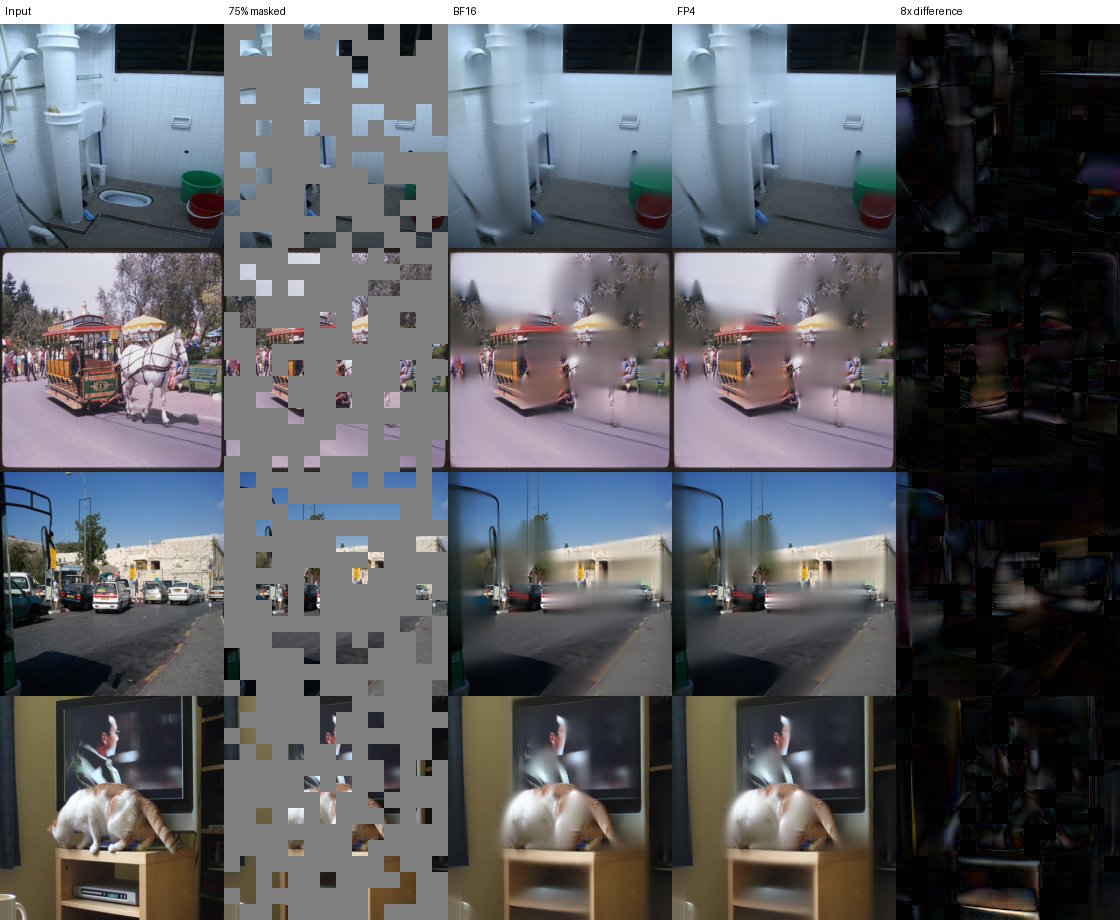
\includegraphics[width=.98\textwidth]
  {../fp4_fa4_reconstruction_20260805/nvmx_fast_report.png}
\caption{Four paired ViT-MAE examples. The right column shows
$8\lvert I_{\mathrm{FP4}}-I_{\mathrm{BF16}}\rvert$; only encoder attention
differs between the BF16 and fast runs.}
\label{fig:mae-reconstruction}
\end{figure}

The aggressive shiftless TK NV/NV control fails on the first sample of every
task, whereas HAO's stabilized NV/NV remains finite. Appendix~\ref{app:nvnv-failure}
shows that the distinction is stabilization, not the use of NVFP4 P itself.
